\pattern{Visitor}

\begin{summary}
The visitor design pattern provides a method of separating an algorithm on an
object and the object’s actual class implementation.  Since the pattern
separates the visitor (operations) from the object structure, it's very easy to
add new visitors as long as the structure remains unchanged.
\end{summary}

Allows you to: \begin{itemize}
    \item add methods to classes of different types without much altering to
        those class.
    \item define external classes that can extend other classes without majorly
        editing them
    \item create a separate visitor concrete class for each type of operation
        and to separate this operation implementation from the objects
        structure.
\end{itemize}

Used when: \begin{itemize}
    \item there are many distinct and unrelated operations
    \item Object structure is not likely to be changed but is very probable to
        have new operations which have to be added
\end{itemize}


\comparison{
    \begin{itemize}
        \item Follows open/close principle
        \item Allows new operations to be added without changing implementation
        \item A visitor can have state
    \end{itemize}
}{
    \begin{itemize}
        \item Does not fit for pattern 1 that updates arguments frequently.
        \item Some non-hierarchy behaviors should not be implemented via
            visitor pattern, since they will be applied to whole system.
    \end{itemize}
}

\begin{nfps}
\item[Maintainability] Center to visitor, increases maintainability
\item[Testability] Each sub class has its own method to debug
\item[Extensibility] Easy to write own method
\item[Reusability] No need to change structures to add new operations
\end{nfps}

\begin{center}
    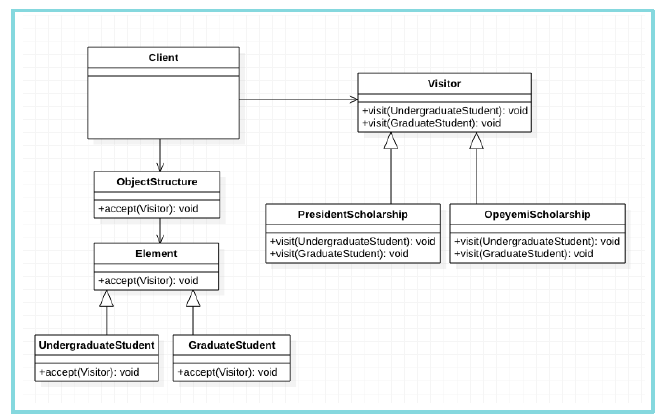
\includegraphics[width=0.5\textwidth]{./visitor}
\end{center}
